\documentclass{beamer}
\usepackage{listings,hyperref,amsmath,graphicx,animate,tikz}
\usetikzlibrary{positioning,shadows,arrows,shapes,calc}
\def\labelenumi\theenumi
\mode<presentation>{\usetheme{Frankfurt}}
\AtBeginSection
{
  \begin{frame}<beamer>
    \frametitle{Outline}
    \tableofcontents[currentsection,currentsubsection]
  \end{frame}
}
\title{Lecture 4: Signal Processing Review}
\author{Mark Hasegawa-Johnson}
\date{ECE 417: Multimedia Signal Processing, Fall 2023}  
\institute{University of Illinois}
\titlegraphic{\includegraphics[width=0.3in]{exp/block-I-primary.png}}
\begin{document}

% Title
\begin{frame}
  \maketitle
\end{frame}

% Title
\begin{frame}
  \tableofcontents
\end{frame}

%%%%%%%%%%%%%%%%%%%%%%%%%%%%%%%%%%%%%%%%%%%%%%%%%%%%%%%%%
\section{Four Fourier Transforms}
\setcounter{subsection}{1}

\begin{frame}
  \frametitle{Four Fourier Transforms}
  \begin{enumerate}
  \item CTFS: Periodic in time, Discrete in frequency
  \item CTFT: Periodic in neither, Discrete in neither
  \item DTFT: Discrete in time, Periodic in frequency
  \item DFT: Discrete in both, Periodic in both
  \end{enumerate}
\end{frame}

\begin{frame}
  \frametitle{Continuous Time Fourier Series: Periodic in time, Discrete in frequency}

  \textbf{Forward Transform:}
  \begin{displaymath}
    X_k = \frac{1}{T_0}\int_{t=0}^{T_0} x(t)e^{-jk\Omega_0 t}dt,~~~\Omega_0=\frac{2\pi}{T_0}
  \end{displaymath}
  \textbf{Inverse Transform:}
  \begin{displaymath}
    x(t) = \sum_{k=-\infty}^\infty X_ke^{jk\Omega_0 t}
  \end{displaymath}
  \textbf{Parseval's Theorem:}
  \begin{displaymath}
    \frac{1}{T_0}\int_{t=0}^{T_0}|x(t)|^2dt=\sum_{k=-\infty}^\infty|X_k|^2
  \end{displaymath}
\end{frame}

\begin{frame}
  \frametitle{Continuous Time Fourier Transform: Periodic in neither, Discrete in neither}
  
  \textbf{Forward Transform:}
  \begin{displaymath}
    X(\Omega) = \int_{-\infty}^\infty x(t)e^{-j\Omega t}dt
  \end{displaymath}
  \textbf{Inverse Transform:}
  \begin{displaymath}
    x(t) = \frac{1}{2\pi}\int_{-\infty}^\infty X(\Omega)e^{j\Omega t}d\Omega
  \end{displaymath}
  \textbf{Parseval's Theorem:}
  \begin{displaymath}
    \int_{-\infty}^{\infty}|x(t)|^2dt=\frac{1}{2\pi}\int_{-\infty}^\infty|X(\Omega)|^2d\Omega
  \end{displaymath}
\end{frame}

\begin{frame}
  \frametitle{Discrete Time Fourier Transform: Discrete in time, Periodic in frequency}

  \textbf{Forward Transform:}
  \begin{displaymath}
    X(\omega) = \sum_{n=-\infty}^\infty x[n]e^{-j\omega n}
  \end{displaymath}
  \textbf{Inverse Transform:}
  \begin{displaymath}
    x[n] = \frac{1}{2\pi}\int_{0}^{2\pi} X(\omega)e^{j\omega n}d\omega
  \end{displaymath}
  \textbf{Parseval's Theorem:}
  \begin{displaymath}
    \sum_{-\infty}^{\infty}|x[n]|^2=\frac{1}{2\pi}\int_{0}^{2\pi}|X(\omega)|^2d\omega
  \end{displaymath}
\end{frame}

\begin{frame}
  \frametitle{Discrete Fourier Transform: Discrete in both, Periodic in both}

  \textbf{Forward Transform:}
  \begin{displaymath}
    X[k] = \sum_{n=0}^{N-1} x[n]e^{-j\frac{2\pi kn}{N}}
  \end{displaymath}
  \textbf{Inverse Transform:}
  \begin{displaymath}
    x[n] = \frac{1}{N}\sum_{k=0}^{N-1} X[k]e^{j\frac{2\pi kn}{N}}
  \end{displaymath}
  \textbf{Parseval's Theorem:}
  \begin{displaymath}
    \sum_{n=0}^{N-1}|x[n]|^2=\frac{1}{N}\sum_{k=0}^{N-1}|X[k]|^2
  \end{displaymath}
\end{frame}



%%%%%%%%%%%%%%%%%%%%%%%%%%%%%%%%%%%%%%%%%%%%%%%%%%%%%%%%%
\section{Impulses}
\setcounter{subsection}{1}

\begin{frame}
  \frametitle{Discrete-Time Impulse}

  \textbf{Definition:}
  \begin{displaymath}
    \delta[n-n_0]=\left\{\begin{array}{ll}
    1&n=n_0\\
    0&\mbox{otherwise}
    \end{array}\right.~~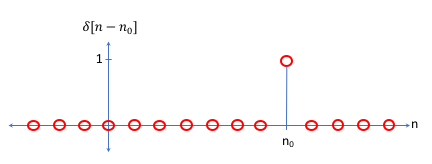
\includegraphics[width=1.5in]{figs/dti_drawing.png}
  \end{displaymath}
      \textbf{Sampling Theorem:}
      \begin{displaymath}
    \sum_{n=-\infty}^\infty\delta[n-n_0]f[n]=f[n_0]
  \end{displaymath}
  \textbf{DTFT of an Impulse:}
  \begin{align*}
    x[n]=\delta[n-n_0]&\leftrightarrow X(\omega)=e^{-j\omega n_0}
  \end{align*}
  \textbf{DFT of a Cosine:}
  \begin{displaymath}
    x[n]=\cos\left(\left(\frac{2\pi a}{N}\right)n\right)\leftrightarrow
    X[k]=\frac{N}{2}\delta[k-a]+\frac{N}{2}\delta[k-(N-a)]
    %~~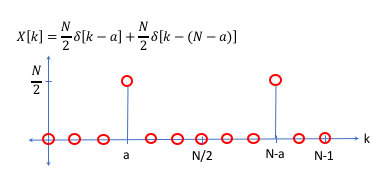
\includegraphics[width=1in]{figs/dti_inverse_drawing.png}
  \end{displaymath}
  \end{frame}

\begin{frame}
  \frametitle{Continuous-Time Impulse}

  \textbf{Definition:}
  \begin{displaymath}
    \delta(t-t_0)=
    \left\{\begin{array}{ll}
    \infty&t=t_0\\
    0&\mbox{otherwise}
    \end{array}\right.~~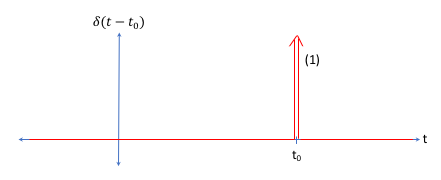
\includegraphics[width=1.5in]{figs/cti_drawing.png}
  \end{displaymath}
  \textbf{Sampling Theorem:}
  \begin{displaymath}
    \int_{t=-\infty}^\infty\delta(t-t_0)f(t)=f(t_0)
  \end{displaymath}
  \textbf{CTFT of an Impulse:}
  \begin{align*}
    x[n]=\delta(t-t_0)&\leftrightarrow X(\Omega)=e^{-j\Omega t_0}
  \end{align*}
  \textbf{CTFT of a Cosine:}
  \begin{displaymath}
    x(t)=\cos(\alpha t)
    \leftrightarrow
    X(\Omega)=\pi\delta(\Omega-\alpha)+\pi\delta(\Omega+\alpha)
    ~~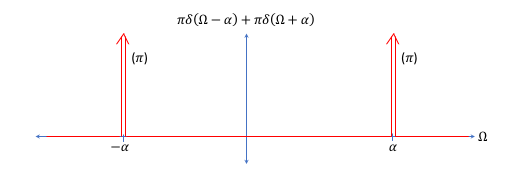
\includegraphics[width=1.5in]{figs/cti_inverse_drawing.png}
  \end{displaymath}
\end{frame}

%%%%%%%%%%%%%%%%%%%%%%%%%%%%%%%%%%%%%%%%%%%%%%%%%%%%%%%%%
\section{Rectangles}
\setcounter{subsection}{1}

\begin{frame}
  \frametitle{DTFT: Rectangle $\leftrightarrow$ Sinc}

  \begin{itemize}
  \item The DTFT of a sinc is a rectangle:
    \begin{displaymath}
      h[n] = \left(\frac{\omega_c}{\pi}\right)\mbox{sinc}(\omega_c n)
      ~~~\leftrightarrow~~~
      H(\omega)=\begin{cases}1&|\omega|<\omega_c\\
      0 & \omega_c<|\omega|<\pi
      \end{cases}
    \end{displaymath}
  \item The DTFT of an even-symmetric rectangle is a sinc-like function, called the
    Dirichlet form:
    \begin{displaymath}
      d_L[n] = \begin{cases}
        1 & |n|\le \frac{L-1}{2}\\
        0 &\mbox{otherwise}
      \end{cases}
      ~~~\leftrightarrow~~~
      D_L(\omega)= \frac{\sin(\omega L/2)}{\sin(\omega/2)}
    \end{displaymath}
  \end{itemize}
\end{frame}

\begin{frame}
  \frametitle{Rectangle $\leftrightarrow$ Sinc}

  \centerline{\includegraphics[width=\textwidth]{exp/rectangles_and_sincs.png}}
\end{frame}

\begin{frame}
  \frametitle{Symmetric and Causal Rectangles}

  The causal rectangular window is:
  \begin{displaymath}
    w_R[n]=\left\{\begin{array}{ll}
    1 & 0\le n\le L-1\\
    0 &\mbox{otherwise}
    \end{array}\right.
  \end{displaymath}
  Its DTFT is:
  \begin{align*}
    W_R(\omega) &= \sum_{n=-\infty}^\infty w_R[n]e^{-j\omega n}
    = \sum_{n=0}^{L-1} e^{-j\omega n} \\
    &= \frac{1-e^{-j\omega L}}{1-e^{-j\omega}}\\
    &= \frac{\sin(\omega L/2)}{\sin(\omega/2)}e^{-j\omega\left(\frac{L-1}{2}\right)}
  \end{align*}
  It's just a delayed version of the symmetric rectangle:
  \begin{align*}
    w_R[n]=d_L\left[n-\frac{L-1}{2}\right] \leftrightarrow
    W_R(\omega) = D_L(\omega)e^{-j\omega\left(\frac{L-1}{2}\right)}
  \end{align*}
\end{frame}

\begin{frame}
  \frametitle{Properties of the Dirichlet form: Periodicity}

  \begin{columns}
    \begin{column}{0.5\textwidth}

      \begin{displaymath}
        D_L(\omega) = \frac{\sin(\omega L/2)}{\sin(\omega/2)}
      \end{displaymath}
      Both numerator and denominator are periodic with period $2\pi$.
    \end{column}
    \begin{column}{0.5\textwidth}
      \centerline{\includegraphics[width=\textwidth]{exp/dirichlet_2pi_period.png}}
    \end{column}
  \end{columns}
\end{frame}

\begin{frame}
  \frametitle{Properties of the Dirichlet form: DC Value}

  \begin{columns}
    \begin{column}{0.5\textwidth}

      \begin{displaymath}      
        D_L(0) = \sum_{n=-\infty}^\infty w[n] = L
      \end{displaymath}
      
    \end{column}
    \begin{column}{0.5\textwidth}
      \centerline{\includegraphics[width=\textwidth]{exp/dirichlet_dc_is_L.png}}
    \end{column}
  \end{columns}
\end{frame}

\begin{frame}
  \frametitle{Properties of the Dirichlet form: Sinc-like}

  \begin{columns}
    \begin{column}{0.5\textwidth}

      \begin{align*}      
        D_L(\omega) &= \frac{\sin(\omega L/2)}{\sin(\omega/2)}\\
        &\approx \frac{\sin(\omega L/2)}{\omega/2}
      \end{align*}
      Because, for small values of $\omega$,
      $\sin\left(\frac{\omega}{2}\right)\approx\frac{\omega}{2}$.

    \end{column}
    \begin{column}{0.5\textwidth}
      \centerline{\includegraphics[width=\textwidth]{exp/dirichlet_and_2_over_omega.png}}
    \end{column}
  \end{columns}
\end{frame}

\begin{frame}
  \frametitle{Properties of the Dirichlet form: Nulls}

  \begin{columns}
    \begin{column}{0.5\textwidth}

      \begin{displaymath}      
        D_L(\omega) = \frac{\sin(\omega L/2)}{\sin(\omega/2)}
      \end{displaymath}
      It equals zero whenever 
      \begin{displaymath}
        \frac{\omega L}{2} = k\pi
      \end{displaymath}
      For any nonzero integer, $k$.
    \end{column}
    \begin{column}{0.5\textwidth}
      \centerline{\includegraphics[width=\textwidth]{exp/dirichlet_with_null_frequencies.png}}
    \end{column}
  \end{columns}
\end{frame}

\begin{frame}
  \frametitle{Properties of the Dirichlet form: Sidelobes}

  \begin{columns}
    \begin{column}{0.5\textwidth}

      Its sidelobes are
      \begin{align*}      
        D_L\left(\frac{3\pi}{L}\right) &= \frac{-1}{\sin(3\pi/2L)}\approx \frac{-2L}{3\pi}\\
        D_L\left(\frac{5\pi}{L}\right) &= \frac{1}{\sin(5\pi/2L)}\approx \frac{2L}{5\pi}\\
        D_L\left(\frac{7\pi}{L}\right) &= \frac{-1}{\sin(7\pi/2L)}\approx \frac{-2L}{7\pi}\\
        & \vdots
      \end{align*}
    \end{column}
    \begin{column}{0.5\textwidth}
      \centerline{\includegraphics[width=\textwidth]{exp/dirichlet_with_peak_frequencies.png}}
    \end{column}
  \end{columns}
\end{frame}

\begin{frame}
  \frametitle{Properties of the Dirichlet form: Relative Sidelobe Amplitudes}

  \begin{columns}
    \begin{column}{0.5\textwidth}

      The \textbf{relative} sidelobe amplitudes don't depend on $L$:
      \begin{align*}      
        \frac{D_L\left(\frac{3\pi}{L}\right)}{D_L(0)} &=
        \frac{-1}{L\sin(3\pi/2L)}\approx \frac{-2}{3\pi}\\
        \frac{D_L\left(\frac{5\pi}{L}\right)}{D_L(0)} &=
        \frac{1}{L\sin(5\pi/2L)}\approx \frac{2}{5\pi}\\
        \frac{D_L\left(\frac{7\pi}{L}\right)}{D_L(0)} &=
        \frac{-1}{L\sin(7\pi/2L)}\approx \frac{-2}{7\pi}\\
        & \vdots
      \end{align*}
    \end{column}
    \begin{column}{0.5\textwidth}
      \centerline{\includegraphics[width=\textwidth]{exp/dirichlet_with_peak_frequencies.png}}
    \end{column}
  \end{columns}
\end{frame}

\begin{frame}
  \frametitle{Properties of the Dirichlet form: Decibels}
  \begin{columns}
    \begin{column}{0.5\textwidth}

      We often describe the relative sidelobe amplitudes in decibels,
      which are defined as
      \begin{align*}      
        20\log_{10}\left|\frac{D_L\left(\frac{3\pi}{L}\right)}{W(0)}\right| &\approx
        20\log_{10}\frac{2}{3\pi}\approx -13\mbox{dB}\\
        20\log_{10}\left|\frac{D_L\left(\frac{5\pi}{L}\right)}{W(0)}\right| &\approx
        20\log_{10}\frac{2}{5\pi}\approx -18\mbox{dB}\\
        20\log_{10}\left|\frac{D_L\left(\frac{7\pi}{L}\right)}{W(0)}\right| &\approx
        20\log_{10}\frac{2}{7\pi}\approx -21\mbox{dB}\\
        & \vdots
      \end{align*}
    \end{column}
    \begin{column}{0.5\textwidth}
      \centerline{\includegraphics[width=\textwidth]{exp/dirichlet_in_decibels.png}}
    \end{column}
  \end{columns}
\end{frame}



%%%%%%%%%%%%%%%%%%%%%%%%%%%%%%%%%%%%%%%%%%%%%%%%%%%%%%%%%
\section{Filtering and Windowing}
\setcounter{subsection}{1}

\begin{frame}
  \frametitle{Filtering and Windowing}

  \begin{itemize}
  \item Filtering: Convolution in time $\leftrightarrow$ Multiplication in frequency
  \item Windowing: Multiplication in time $\leftrightarrow$ Convolution in frequency
  \end{itemize}
\end{frame}

\begin{frame}
  \frametitle{Filtering: Convolution in time $\leftrightarrow$ Multiplication in frequency}

  \begin{align*}
    Y(\omega)=H(\omega)X(\omega) \leftrightarrow y[n]&=h[n]\ast x[n]\\
    &= \sum_m h[m]x[n-m] \\
    &= \sum_m h[n-m]x[m]
  \end{align*}
\end{frame}

\begin{frame}
  \frametitle{Windowing: Multiplication in time $\leftrightarrow$ Convolution in frequency}

  \begin{align*}
    y[n]=w[n]x[n] \leftrightarrow Y(\omega)&=\frac{1}{2\pi}W(\omega)\ast X(\omega)\\
    &= \frac{1}{2\pi}\int_0^{2\pi}W(\theta)X(\omega-\theta)d\theta\\
    &= \frac{1}{2\pi}\int_0^{2\pi}W(\omega-\theta)X(\theta)d\theta
  \end{align*}
\end{frame}

%%%%%%%%%%%%%%%%%%%%%%%%%%%%%%%%%%%%%%%%%%%%%%%%%%%%%%%%%
\section{Conclusion}
\setcounter{subsection}{1}

\begin{frame}
  \frametitle{Conclusion}
  \begin{enumerate}
  \item Periodic in time $\leftrightarrow$ Discrete in frequency
  \item Discrete in time $\leftrightarrow$ Periodic in frequency
  \item Impulse in time $\leftrightarrow$ Complex exponential in frequency
  \item Complex exponential in time $\leftrightarrow$ Impulse in frequency
  \item Sinc in time $\leftrightarrow$ Rectangle in frequency
  \item Rectangle in time $\leftrightarrow$ Sinc in frequency
  \end{enumerate}
\end{frame}

\end{document}

